\documentclass[12pt]{article}
 
\usepackage[margin=.95in]{geometry} 
\usepackage{amsmath,amsthm,amssymb, graphicx, multicol, array}
 
\newcommand{\N}{\mathbb{N}}
\newcommand{\Z}{\mathbb{Z}}
 

\begin{document}
 
\title{SDS383C Final Project Report \\ \textbf{Inferring Causal Impact Using Bayesian Structural Time-series Models}} 
\author{Brodersen, K., Gallusser, F., Koehler, J., Remy, N., Scott, S.\\Reproduced by Juliette Franqueville
}
\maketitle

\begin{abstract}
    Identifying the most efficient market interventions (such as advertising campaigns, product launches, introduction of a new features, etc) are important for companies to develop competitive advantages. The goal of this paper is to provide a methodology for inferring whether a past market intervention  had an effect on a metric of interest (such as sales, revenue, etc). In this paper, the authors present the model available their R package, ``CausalImpact''. The model comprises of a Bayesian Structural Time Series Model (BSTS) that is used to predict the metric of interest had no market intervention happened. The prediction is then compared to the observed data after the intervention. The causal impact is the difference between the observed and predicted data. The authors provide examples using simulated and empirical data. In this replication, I explain how the model is structured, show an example for how spike-and-slab priors work, and use a Kalman smoother to simulate the state vector in the BSTS model. However, I was not able to fully replicate their model, so I also use their R package to replicate some of the plots present in the original paper.
\end{abstract}

\section{Introduction}
\subsection{Problem Statement}
The paper I chose  presents a Bayesian methodology for inferring causal impact of market interventions on a metric of interest. A market intervention may be the launch of an advertising campaign, the release of a new product, a feature change in a product, or others. It is desirable for companies to understand whether a market intervention has a positive, negative, or insignificant effect on a given metric, such as number of sales, revenue generated, number of users acquired, etc. \\

The causal impact of a treatment is defined as the difference between the observed metric (i.e. sales, number of users acquired, etc) and the metric that would have been observed had no treatment been introduced. This paper deals with time series, so the causal impact is the difference between the observed time series (i.e. sales, number of users acquired as a function of time) and the time series that would have been observed with no market intervention. The main goals of this paper are therefore to 1) predict the time series that would have been observed with no market intervention - this is called the ``counterfactual'' and 2) compare this prediction with the observed time series, where a market intervention was conducted.  A key concept in this paper is that control time-series, such as time-series for other regions where no market intervention was introduced, can be used to predict the counterfactual.

\subsection{Previous Methods}
A typical approach for performing causal inference are ``difference-in-differences'' (DD) methods. DD models a usually based on a linear model between control and treatments groups. Figure \ref{dd} describes a simple example using data I simulated. A control group (for example, sales data from another region) time-series is  available. The treatment group undergoes a  market intervention event. We can model the treatment time series as a linear model of the control time series (in the simulation, I used $y_t = x_t + 500 + \varepsilon_t$, where $y_t$ and $x_t$ are the treatment and control data points at time $t$, respectively.). Using the linear relationship inferred from pre-market intervention data and the post-intervention control group data, the counterfactual treatment time-series can be predicted. The causal impact is then the difference between the observed treatment and predicted treatment time-series post market intervention. 

\begin{figure}[!h]
    \centering
    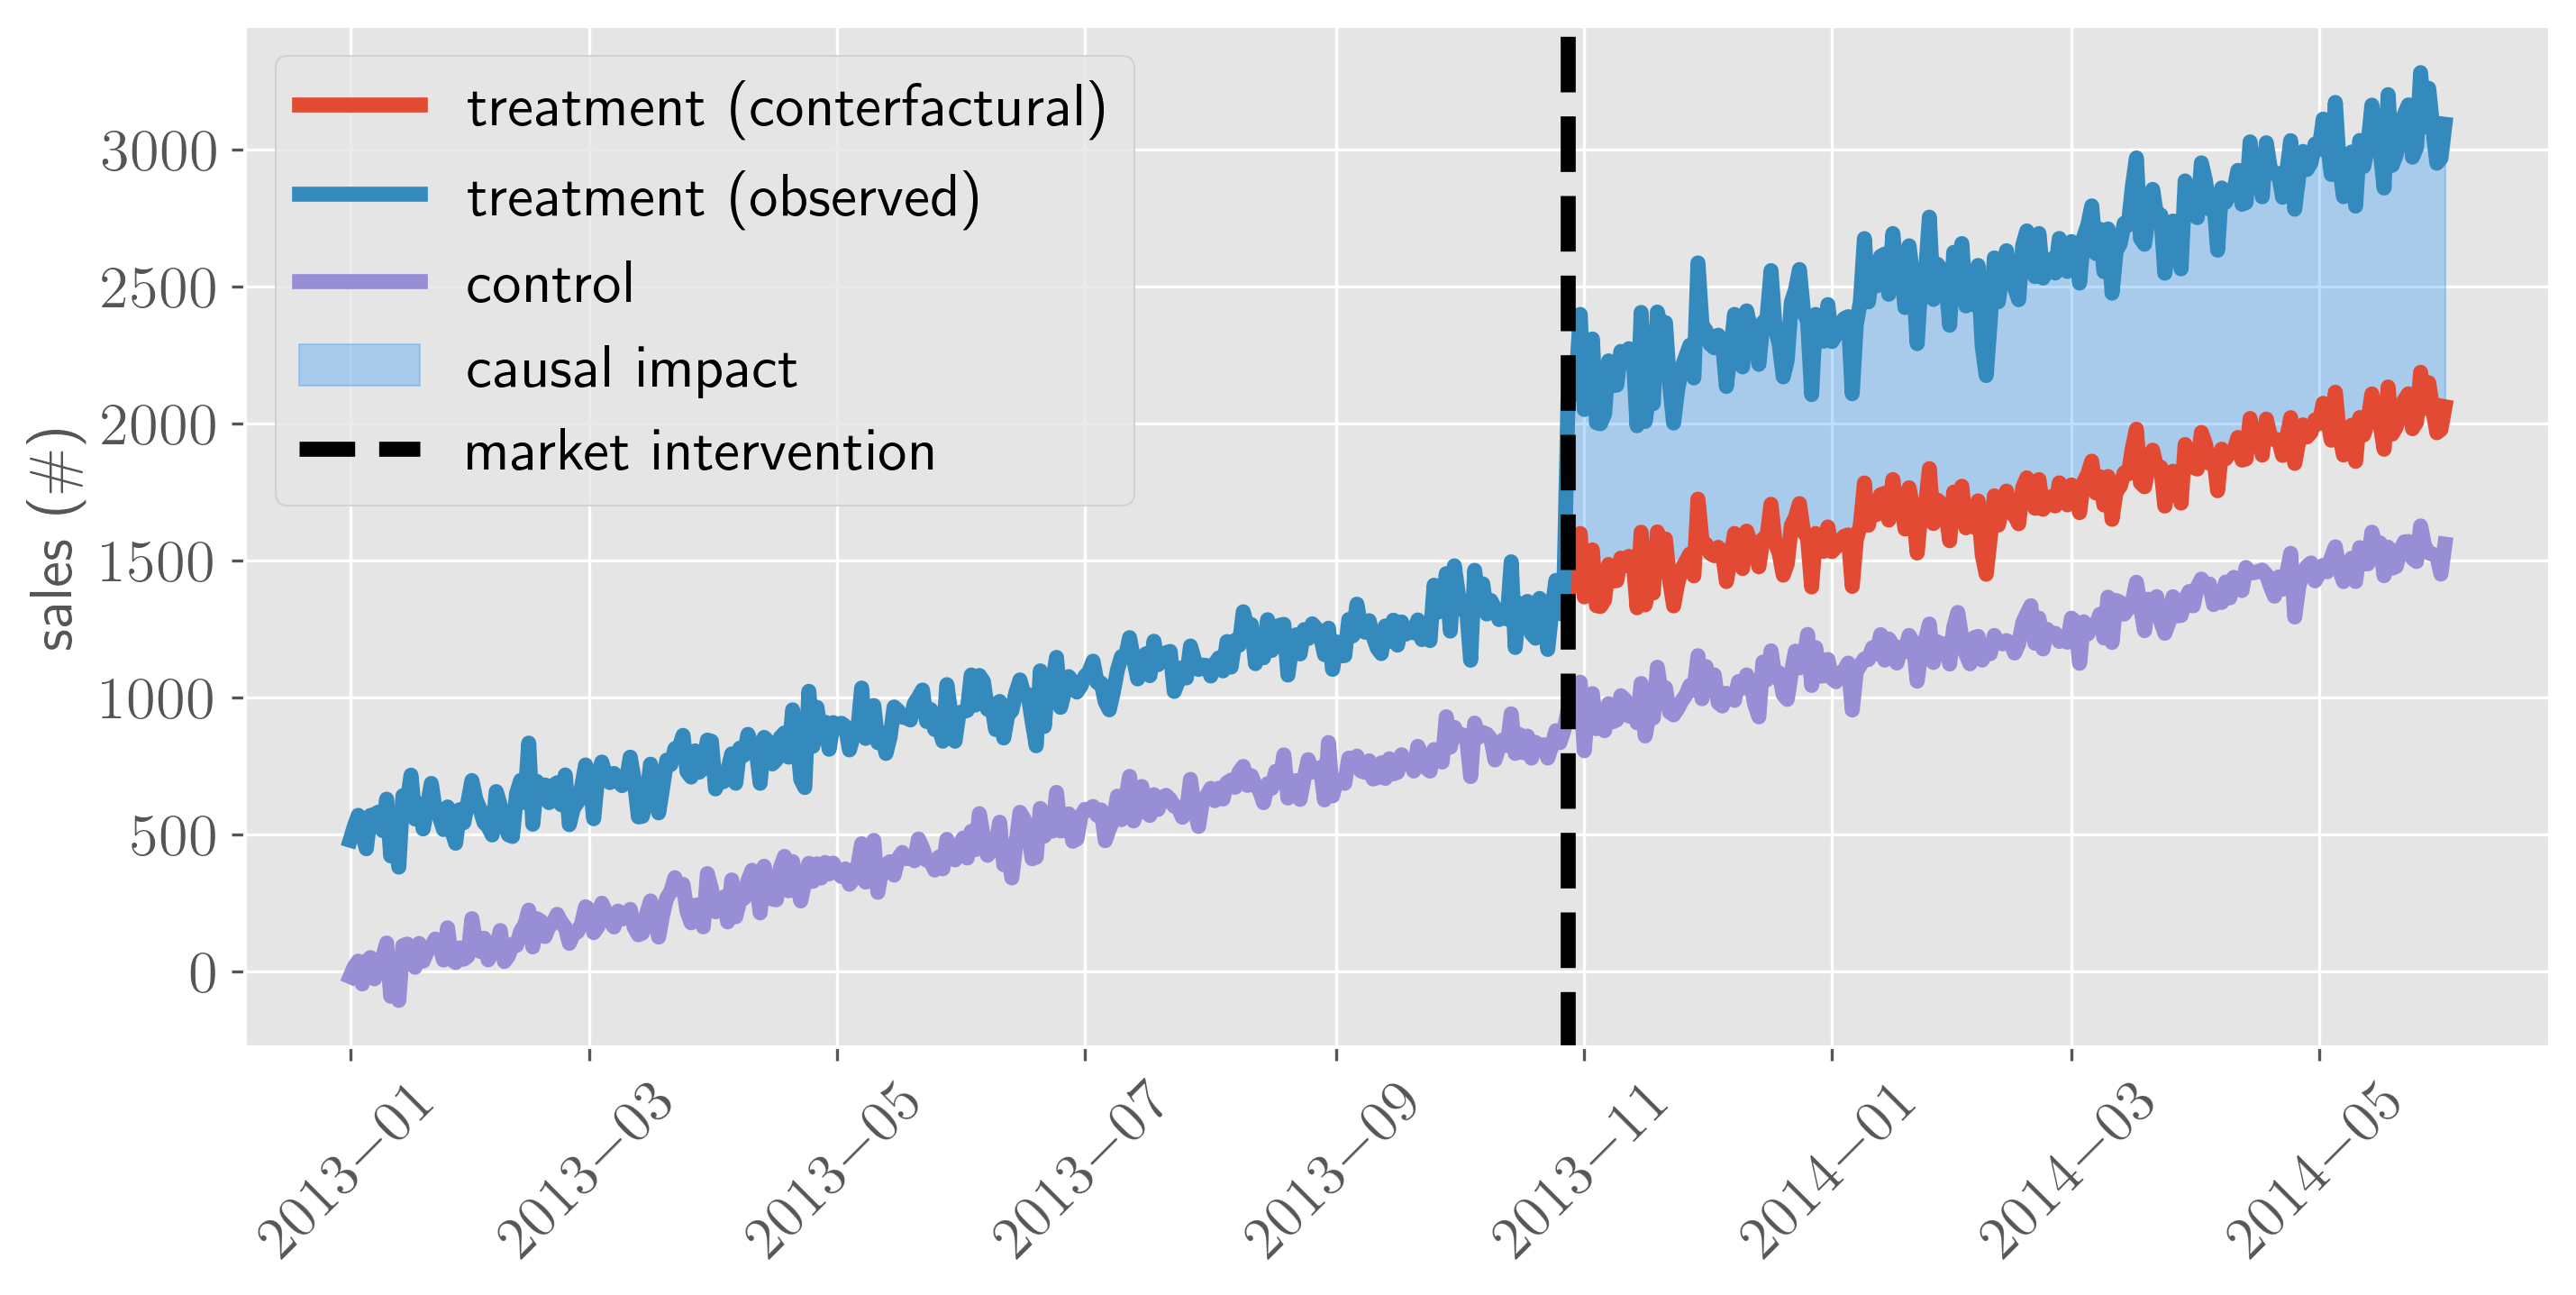
\includegraphics[scale=.6
    ]{../figures/dd.png}
    \caption{Illustration of a DD approach for inferring causal inference. }
    \label{dd}
\end{figure}

There are several limitations associated with this type of approach that this paper seeks to address. For example, DD models are generally not very flexible. Regression coefficients are usually static, which may not be a suitable assumption if they are evolving in time. The authors also wish to avoid using some of the variable selection methods that DD models use. For example, Lasso regression has been used for variable selection \cite{belloni2015program}, but this approach does not take uncertainty about which predictors to use and their coefficients, unlike Bayesian methods.

\subsection{Bayesian Structural Time-series models}
Bayesian Structural Time-series (BSTS) models are very flexible state-space models for time-series data. In fact, all ARIMA models can be specified in this manner. BSTS models can also account for dynamic regression coefficients. A BSTS model is specified as follows:

\begin{align} 
y_t &= \boldsymbol{Z_}t^T\boldsymbol{\alpha}_t + \varepsilon_t\\ \label{eq}
\boldsymbol{\alpha}_{t+1} &= \boldsymbol{T}_t \boldsymbol{\alpha}_t + \boldsymbol{R}_t \boldsymbol{\eta}_t \label{eq1}
\end{align}
Where $\varepsilon_t \sim \mathcal{N}(0, \sigma^2)$ and 
$\eta_t \sim \mathcal{N}(0, \boldsymbol{Q}_t)$. $ \boldsymbol{Q}_t$ is a $p \times p$ matrix, which can be diagonal or not. The first line is the observation equation, and the second is the state equation. $y_t$ is the observed response (scalar), while $\boldsymbol{\alpha}_t$ is a hidden state (scalar or vector, not observed). $\boldsymbol{Z}_t$ is a $p \times n$ matrix, which can for example contain covariates for control groups or rows of 1s, depending on how the model is structured.  $\boldsymbol{T}_t$ is a $p \times p$ ``transition matrix'' and $\boldsymbol{R}_t$ is a $p \times p$ ``control matrix''. Both matrices are populated based on the model. Some common, simple forms of models expressed in this format are shown below. \\

\subsubsection{AR(1) Model}

An AR(1) model  can be written as a BSTS model using:

\begin{align}
    y_t &= \mu_t + \varepsilon_t \\
    \mu_{t+1} &= \phi \mu_t + \eta_t
\end{align}

Which can be re-written in the same format as equations \label{eq} and \label{eq1} by setting $\mu_t = \alpha_t$, $\mu_{t+1} = \alpha_{t+1}$, $Z_t^T = 1$, $T_t = \phi$, $R_t = 1$.


\subsubsection{Local Level}
A local level  can be written as:
\begin{align}
    y_{t} &= \mu_t + \varepsilon_t \\
    \mu_{t+1} &= \mu_t + \eta_t 
    \end{align}

Which can be re-written in the same format as equations \label{eq} and \label{eq1} by setting $\mu_t = \alpha_t$, $\mu_{t+1} = \alpha_{t+1}$, $Z_t^T = 1$, $T_t = 1$, $R_t = 1$.

\subsubsection{Linear Regression (Static Coefficients)}\label{linreg}
A linear regression can be written as:

\begin{align}
    y_{t} &= x_t\beta + \varepsilon_t\\
\end{align}

Which can be re-written in the same format as equations \label{eq} and \label{eq1} by setting $\alpha_t=1$,  $Z_t^T = x_t\beta$.

\subsubsection{Linear Regression (Dynamic Coefficients)}
A linear regression with dynamic coefficients can be written as:

\begin{align}
    y_{t} &= x_t\beta_t + \varepsilon_t\\
    \beta_{t+1} &= \beta_t + \eta_t
\end{align}

Which can be re-written in the same format as equations \label{eq} and \label{eq1} by setting $\beta_t = \alpha_t$, $\beta_{t+1}=\alpha_{t+1}$, $Z_t^T = x_t$, $T_t = 1$, $R_t = 1$.\\

Other state-space models not explicitly  listed include seasonal models, local linear trends, semi-local linear trends, etc. To allow for more flexibility, state components can be assembled by concatenating their observation and hidden state vectors $\boldsymbol{Z}_t$ and $\boldsymbol{\alpha}_t$ and re-arranging other matrices ($\boldsymbol{R}_t, \boldsymbol{T}_t$) as elements in block diagonal matrices. A concrete example showing how to assemble different models is shown in section \ref{toy}.




\section{Methods}
\subsection{Spike-and-Slab Priors}
The paper uses spike-and-slab priors for static regression coefficients (that is, coefficients in \ref{linreg}). Specifying spike-and-slab priors over regression coefficients is essentially a Bayesian method for variable selection. Variable selection is the process of choosing only some of the covariates available. Lasso is a typical frequentist method for variable selection in regressions. For a static regression component with multiple $\beta_i$ coefficients formulated as:

\begin{align}
    y_t &=  \boldsymbol{X}_t\boldsymbol{\beta} + \varepsilon_t\\
     \varepsilon_t &\sim \mathcal{N}(0, \sigma^2)
\end{align}

A spike-and-slab prior has the form:

\begin{align}
    \beta_i \sim (1-\pi_i)\delta_0 + \pi_i\mathcal{N}(0, \tau^2\sigma^2)
\end{align}


Where $\pi_i \in [0, 1]$, and $\delta_0$ is the Dirac delta function. With $\pi_i = 0.5$, $\sigma^2 = 1$, $\tau^2 = 1$, this distribution is shown in Figure \ref{prior}



\begin{figure}[!h]
    \centering
    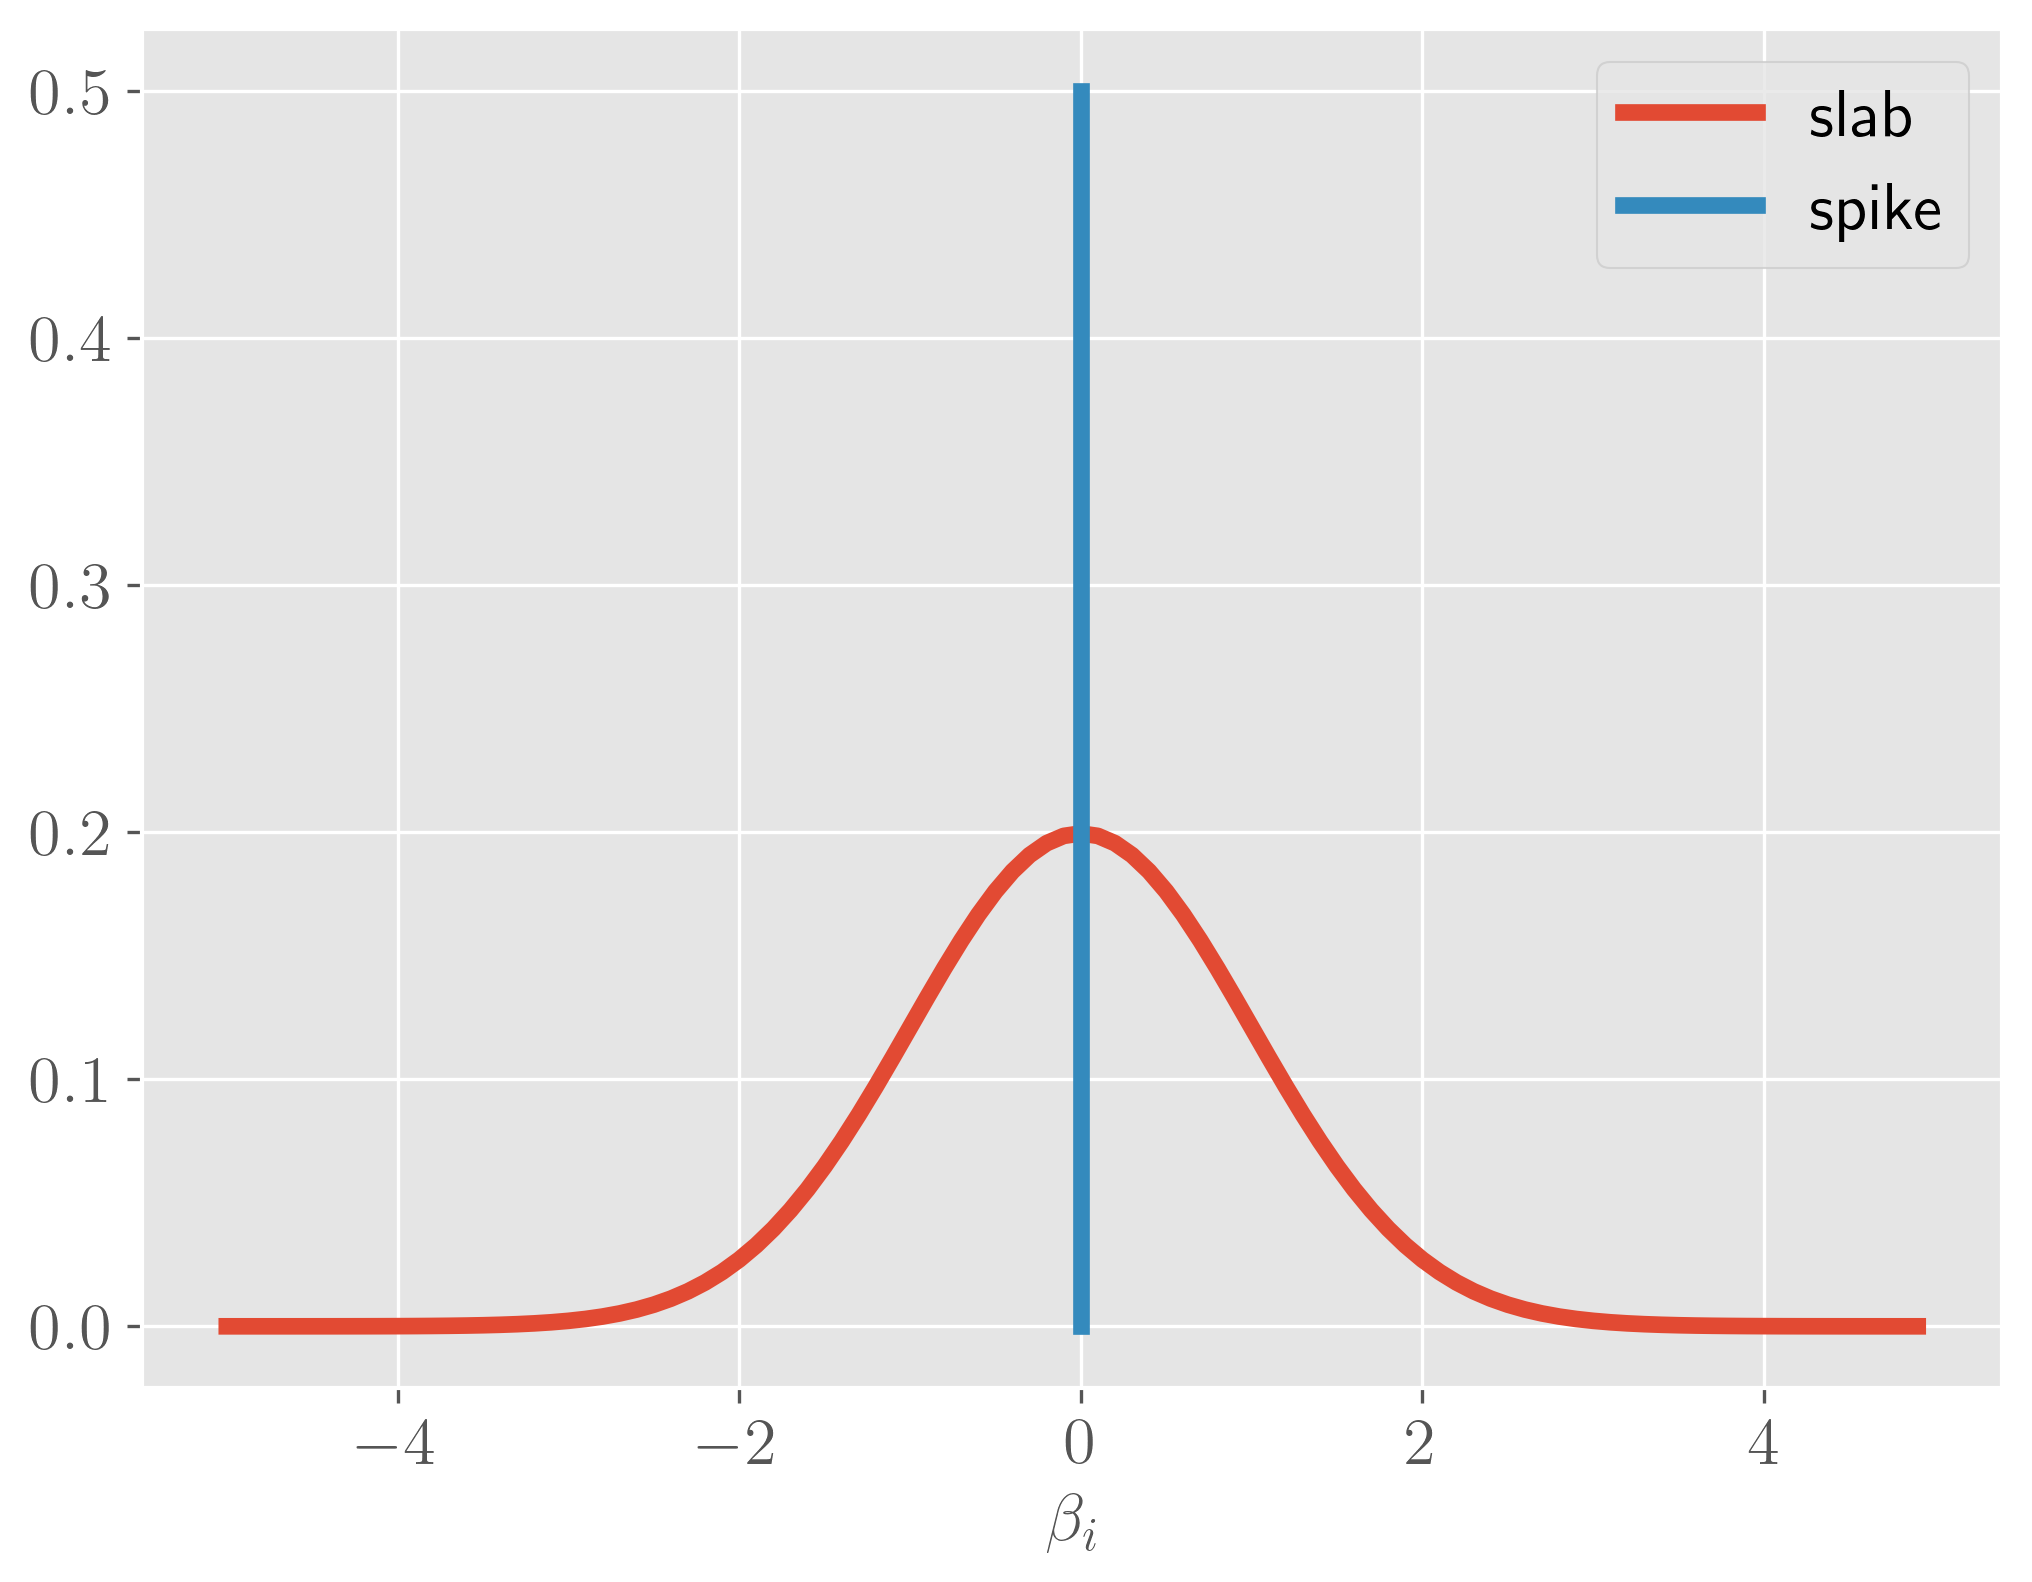
\includegraphics[scale=.6
    ]{../figures/spike.png}
    \caption{Spike-and-slab prior illustration.}
    \label{prior}
\end{figure}

I reproduced this aspect of the paper by creating a simulated dataset using:

\begin{align*}
    y_t& = x_{1, t}\beta_1 + x_{2, t}\beta_2 + \varepsilon_t\\
    \varepsilon_t &\sim \mathcal{N}(0, \sigma^2)
\end{align*}

With $\beta_1 = 10$,  $\beta_2 = 0.05$, and $\sigma^2 = 4$. Figure \ref{toydata} shows the dataset created. 

\begin{figure}[!h]
    \centering
    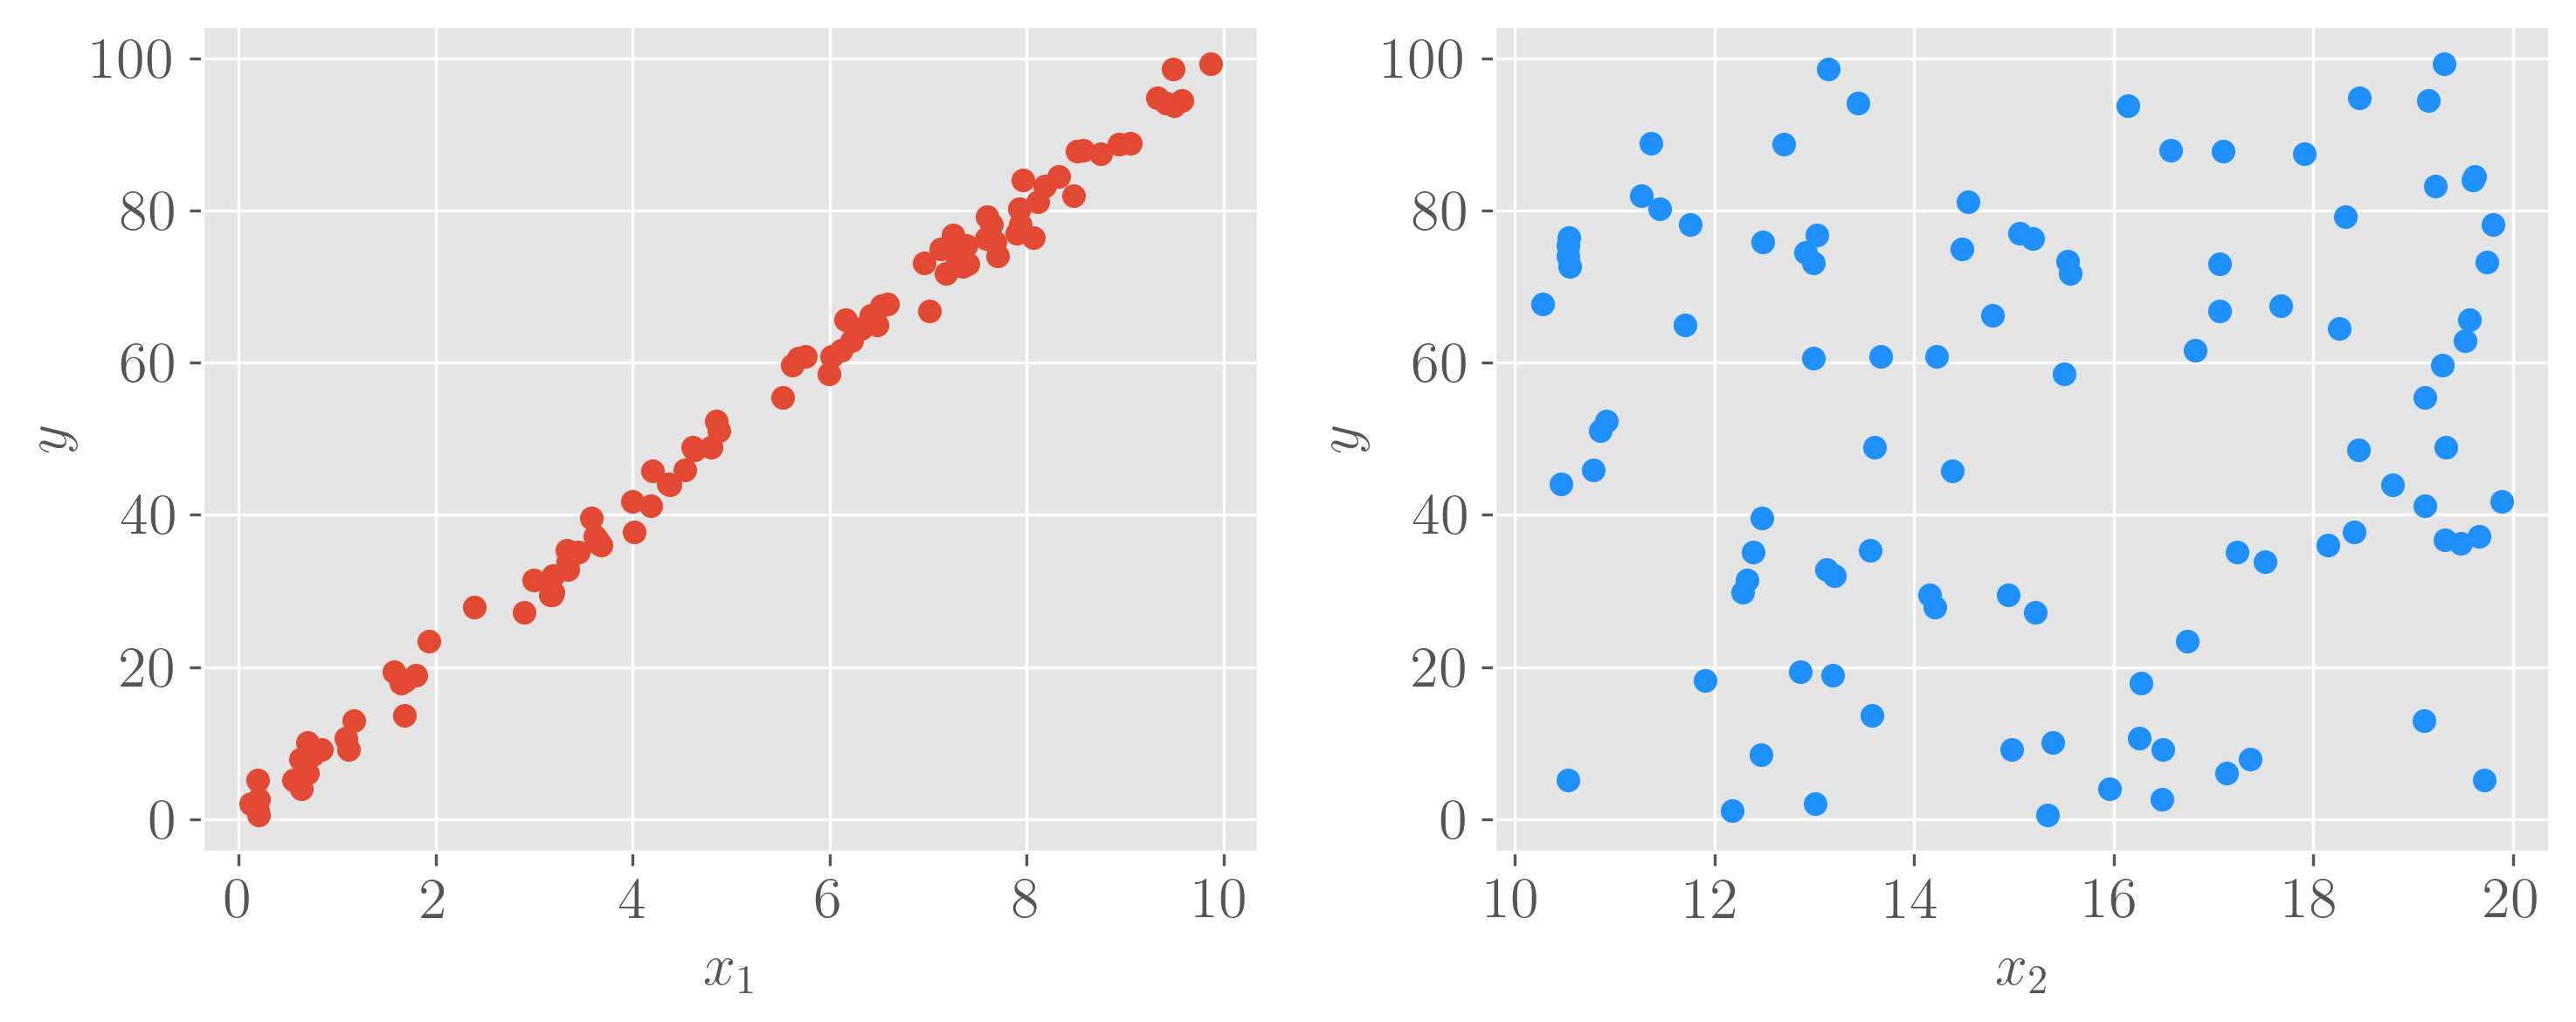
\includegraphics[scale=.6
    ]{../figures/toydata.png}
    \caption{Simulated data for reproduction of regression coefficient inference using spike-and-slab priors.}
    \label{toydata}
\end{figure}

I used the following priors:

\begin{align*}
    \tau^2 &\sim IG(1, s^2/2)\\
    \sigma^2 &\sim IG(\alpha_1, \alpha_2)\\
    \pi_i &\sim Bernoulli(\theta)\\
    \theta & \sim Beta(a, b)
\end{align*}

The conditional posteriors were (note that I checked my answers against \cite{andrade2020disjunct}):

\begin{align}
    P(\theta|\boldsymbol{\pi}) &\sim Beta(a + \sum_{i=1}^p \pi_i, b + \sum_{i=1}^p [1-\pi_i])\\
    z_i &\sim Bernoulli(\pi_i)\\
    P(\boldsymbol{\beta}|\sigma^2, \tau^2) &= \begin{cases}
     \mathcal{N}\left(\left[\boldsymbol{X}^T\boldsymbol{X} \frac{1}{\sigma^2} + \boldsymbol{I}\frac{1}{\sigma^2\tau^2}\right]^{-1}\boldsymbol{X}^T \boldsymbol{y} \frac{1}{\sigma^2}, \left[\boldsymbol{X}^T\boldsymbol{X} \frac{1}{\sigma^2} + \boldsymbol{I}\frac{1}{\sigma^2\tau^2}\right]^{-1}\right)& \text{if } z_i = 1\\
    0             & \text{if } z_i = 0
\end{cases}\\
P(\sigma^2|\boldsymbol{\beta}) &\sim IG\{\alpha_1 + n/2, \alpha_2 + \frac{1}{2}(\boldsymbol{y}-\boldsymbol{X}\boldsymbol{\beta})^T(\boldsymbol{y}-\boldsymbol{X}\boldsymbol{\beta})\} \\
P(\tau^2|\boldsymbol{\beta}, \boldsymbol{\pi}) &\sim IG(1/2 + 1/2\sum_1^{p}\pi_i, s^2/2 + \boldsymbol{\beta}^T\boldsymbol{\beta}/2\sigma^2)\\
\end{align}
And finally, $\pi_i$ is updated using 

\begin{align}
    1-\pi_i = \frac{1-\theta}{(\sigma^2\tau^2)^{-1/2}\text{exp}\left(\frac{\sum_1^n x_j(y_j - X_{-i, j}\beta_{-i, j})}{2\sigma^2(\sum_1^n x_j^2 + 1/\sigma^2)}\right)  \left(\frac{\sigma^2}{\sum_1^n x_j^2 + 1/\sigma^2}\right)^{1/2}\theta   + (1-\theta)  }
\end{align}

Where $\boldsymbol{X}_{-i}$ and $\boldsymbol{\beta}_{-i}$ are $\boldsymbol{X}$ and $\boldsymbol{\beta}$ with the column and row corresponding to $i$ removed, respectively. At each iteration, $z_i$ is drawn from a Bernoulli distribution with $\pi_i$ parameter. Figure \ref{post} below show the posteriors for $\beta_1$ and $\beta_2$ from the Gibbs sampling algorithm:

\begin{figure}[!h]
    \centering
    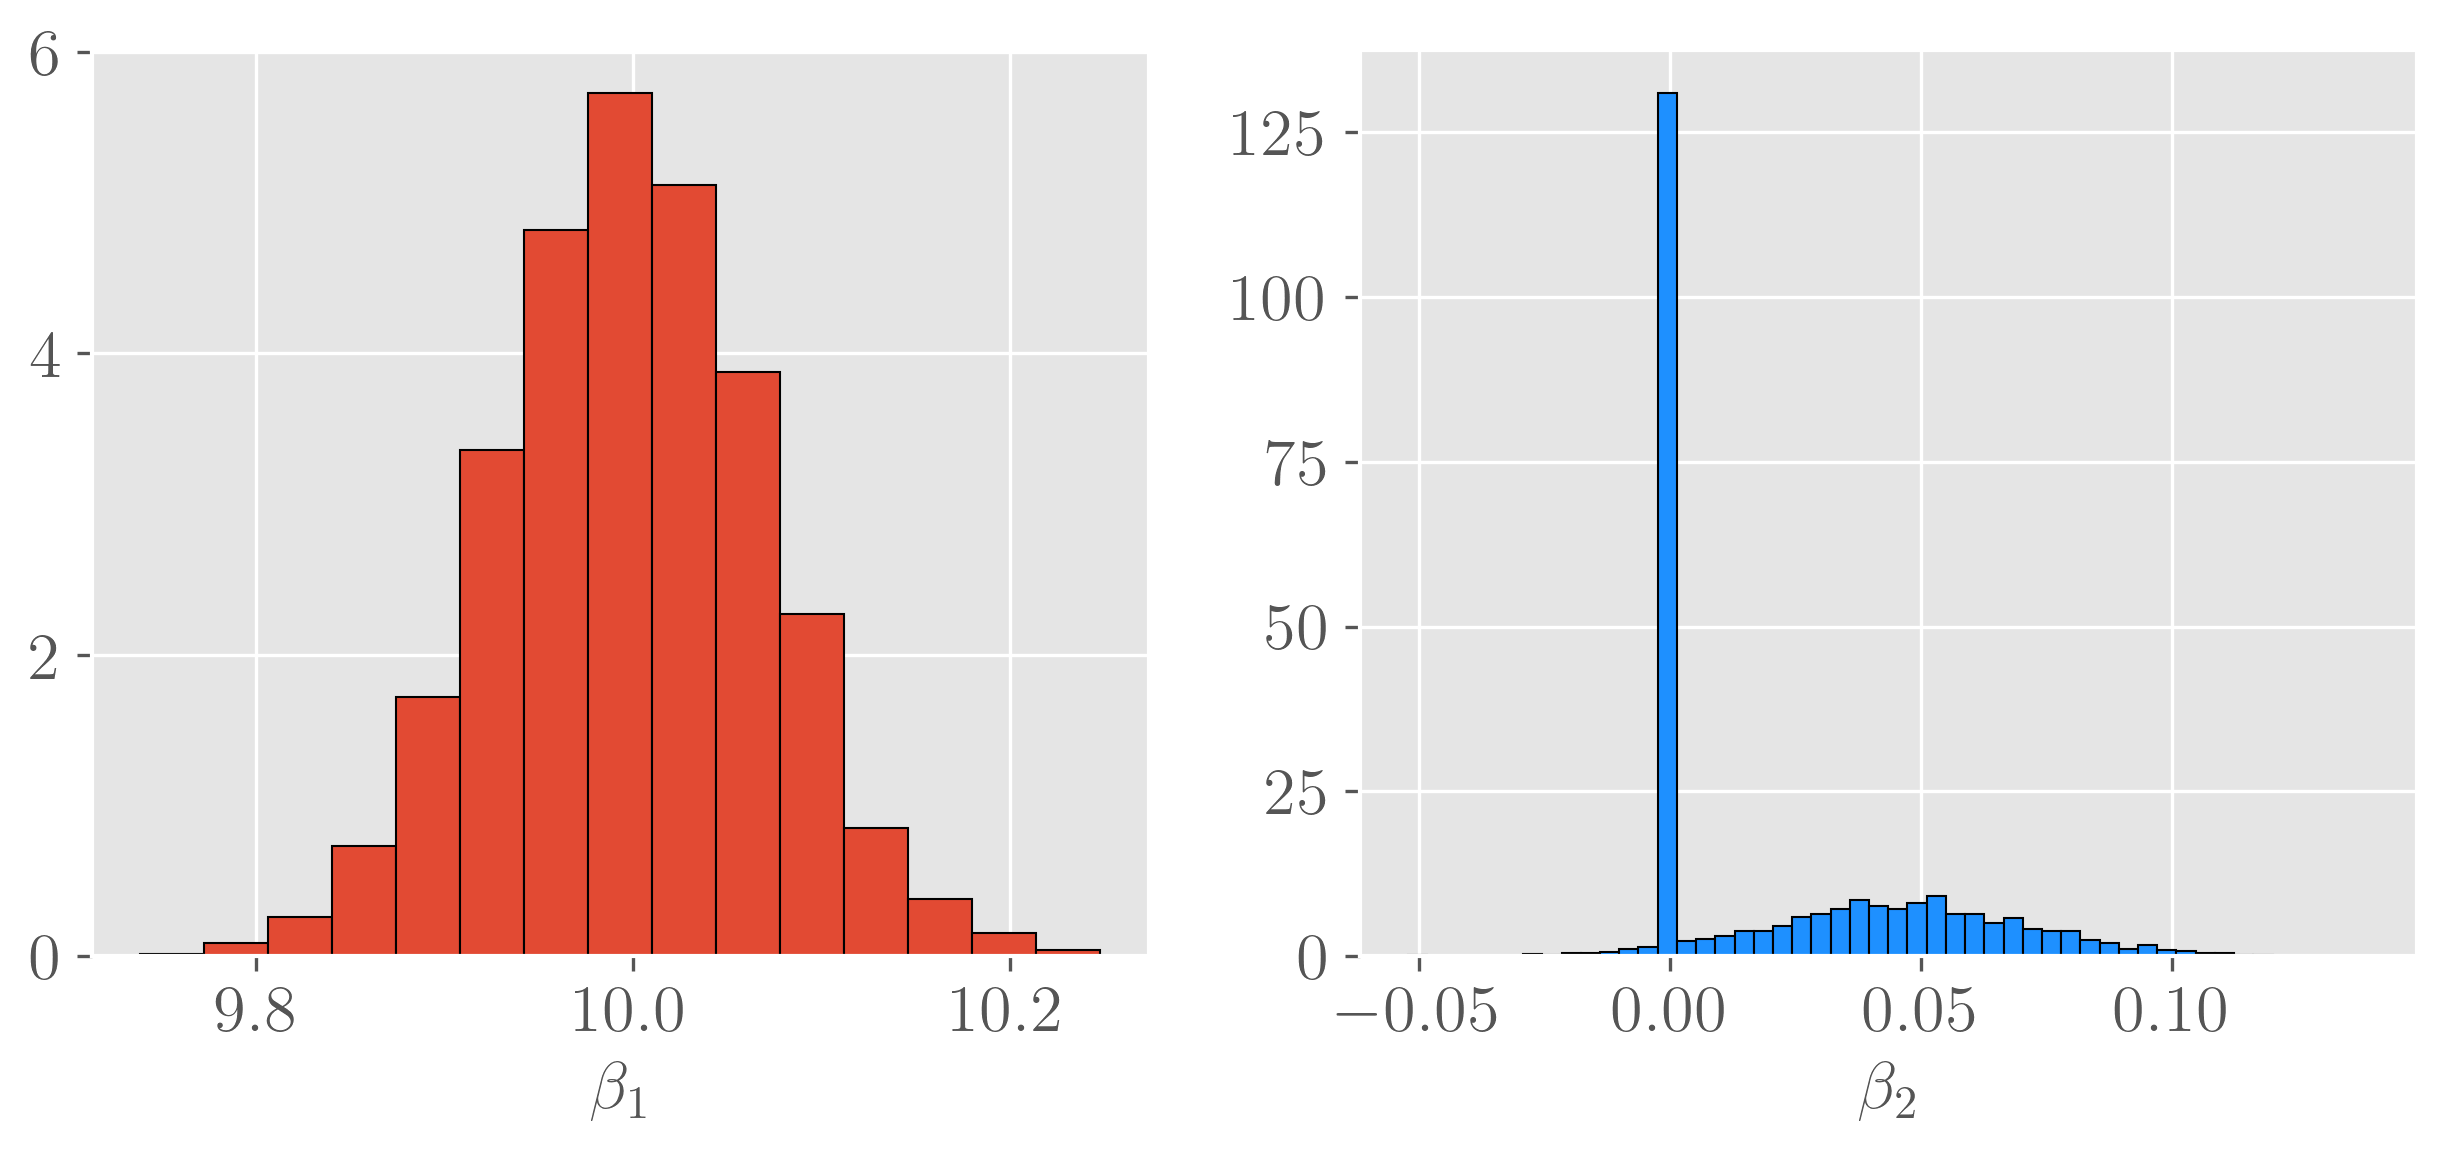
\includegraphics[scale=.6
    ]{../figures/posteriors.png}
    \caption{Posteriors for $\beta_1$ and $\beta_2$.}
    \label{post}
\end{figure}

As expected, the posterior for $\beta_1$ does not exhibit a strong spike, but the posterior for  $\beta_2$ exhibits a strong spike at 0 (its MAP is 0). This suggests that $\beta_1$ needs to be included in the model, but $\beta_2$ does not. Formally, variable selection from those posteriors can be done using the posterior inclusion probabilities ($\pi_i$). I reproduced this aspect of the paper in isolation, but of course, this step happens in combination with sampling the other parameters in the model (e.g. local level, dynamic regression coefficients, etc). Note that there may be some differences between what I implemented and what the paper implemented (due to the fact that some details were omitted in the paper), but the general approach is the same. 

\subsection{Kalman Filtering and Smoothing}

The state vector $\boldsymbol{\alpha}_t$ in BSTS models is unobserved. However, this vector must be estimated to  forecast the counterfactual time series. A natural way to simulate the state vector is to use Kalman filtering and smoothing. The paper used an improved algorithm from Durbin and Koopman \cite{durbin2002simple}. However, given that I was new to Kalman filtering, I only had time to get familiar/implement basic algorithms, which are described below. \\

\subsubsection{Kalman Filtering}\label{kalman}
The aim of Kalman filtering is to predict $\boldsymbol{\alpha}_{t}|\boldsymbol{y_{1:t}}$, that is, to predict the state vector at time $t$ given observed data up to  $t$. There are two steps in Kalman filtering: updating and predicting. The update step is:

\begin{align*}
    \alpha_{t|t-1} &= T_t \alpha_t\\
    P_{t|t-1} &= T_t P_{t-1|t-1} T_t^T + Q_t
\end{align*}

The predicting step is:
\begin{align*}
    v_t &= y_t - Z_t^T \alpha_{t|t-1}\\
    F_t &= Z_t^T P_{t|t-1} Z_t + \sigma^2\\
    K_t &= P_{t|t-1} Z_t^T F_t^{-1}\\
    \alpha_{t|t} &= \alpha_{t|t-1} + K_t v_t\\
    P_{t|t} &= (I - K_t Z_T^T)P_{t|t-1}
\end{align*}

$ \alpha_{t|t}$ is the predicted mean for the state vector, and $P_{t|t}$ is the covariance matrix. 

\subsubsection{Kalman Smoothing}
Kalman Smoothing is an algorithm that comprises of a forward pass (which is the same as Kalman filtering), and a backward pass. The backward pass computes smoothed estimates for the state vector. I used the Rauch–Tung–Striebel algorithm for Kalman smoothing. The backward pass is done using:

\begin{align*}
    \alpha_{t|n} &= \alpha{t|t} + C_t(\alpha_{t+1|n} - \alpha_{t+1|t})\\
    P_{t|n} &= P_{t|t} + C_t(P_{t+1|n} - P_{t+1|t})C_t^T
\end{align*}

Where $C_t = P_{t|t}F_{t+1}P_{t+1|t}^{-1}$. $\alpha_{t+1|n}$, $\alpha_{t+1|t}$, $P_{t+1|n}$, $P_{t+1|t}$ are obtained from the forward pass previously run. 

\subsubsection{Forecasting}
The goal of the paper is to forecast the counterfactual time series to compare it to observed data. After using the Kalman Smoothing algorithm, data is forecast using:

\begin{align*}
    \alpha^*_{t + 1}& =  T_{t} \alpha_{t|t} \\
    P^*_{t + 1}& =  T_{t} P_{t|t} T_t^T + Q_t\\
    y^*_{t + 1} &= Z_{t + 1}^T \alpha^*_{t + 1}\\
    \sigma^{2*}_{t + 1} &= Z_{t + 1}^T P^*_{t + 1}Z_{t + 1} + \sigma^2\\
\end{align*}

For the first time step, and then for $d > 1$:


\begin{align*}
    \alpha^*_{t + d}& =  T_{t} \alpha^*_{t + d -1} \\
    P^*_{t + d}& =  T_{t} P^*_{t + d - 1} T_t^T + Q_t\\
    y^*_{t + d} &= Z_{t + 1}^T \alpha^*_{t + d}\\
    \sigma^{2*}_{t + d} &= Z_{t + d}^T P^*_{t + d}Z_{t + d} + \sigma^2\\
\end{align*}


\subsection{Gibbs Sampling}
The paper uses a Gibbs sampler that comprises of the following steps:
\begin{itemize}
    \item Sample from $P(\boldsymbol{\alpha}|\boldsymbol{y}, \boldsymbol{\theta}, \boldsymbol{\beta},  \boldsymbol{\sigma^2_{\beta}})$ using the Kalman smoother algorithm from \cite{durbin2002simple}
    \item Sample from $\boldsymbol{\theta}\sim P(\boldsymbol{\theta}|\boldsymbol{y}, \boldsymbol{\beta},  \boldsymbol{\sigma^2_{\beta}}, \boldsymbol{\alpha})$
    \item Sample from $P(\boldsymbol{\beta},\boldsymbol{\sigma^2_{\beta}}|\boldsymbol{\alpha}, \boldsymbol{\theta}, \boldsymbol{y})$
\end{itemize}

Where $\boldsymbol{\beta}$ are static regression coefficients (with spike-and-slab priors placed on them) and $\boldsymbol{\sigma^2_\beta}$ their associated variances. $\boldsymbol{\theta}$ is the vector of remaining parameters to be estimated, and $\boldsymbol{\alpha}$ is the state vector. The Gibbs sampling algorithm yields to the stationary distribution $P(\boldsymbol{\alpha}, \boldsymbol{\theta}, \boldsymbol{\beta},  \boldsymbol{\sigma^2_{\beta}}|\boldsymbol{y})$.

\section{Example with Simulated Data}\label{toy}
The paper features an demonstration of their method using simulated data. I was unable to fully replicate their method, so I only implemented the Kalman smoothing step described in section \ref{kalman}, assuming that all parameters were known. Note that the example did not comprise of a static regression, so I did not use my spike-and-slab code in this context. I replicated some of the other plots using the authors' R package, which is described in detail in a previous paper \cite{scott2014predicting}. I tried to match the simulated data as closely as possible, but some details in the paper were left out.

\subsection{Data Simulation}\label{dataset}
The BSTS model at hand comprises of a dynamic regression with two covariates and a local level. The covariates could for example represent revenue in other regions that did not receive the maket intervention. The BSTS model is structured as follows:

\begin{align}
y_t &= \begin{bmatrix} \label{q1}
1 & 0 & 0\\
0 & x_{t, 1} & 0\\
0 & 0 & x_{t, 2}
\end{bmatrix} \begin{bmatrix}
\mu_{t} \\
\beta_{t, 1} \\
\beta_{t, 2} \\
\end{bmatrix} +
\varepsilon_{t} \\
\begin{bmatrix} \label{q2}
\mu_{t+1} \\
\beta_{t+1, 1} \\
\beta_{t+1, 2} \\
\end{bmatrix} &=  \begin{bmatrix}
1 & 0 & 0\\
0 & 1 & 0\\
0 & 0 & 1
\end{bmatrix}  \begin{bmatrix}
\mu_{t} \\
\beta_{t, 1} \\
\beta_{t, 2} \\
\end{bmatrix} + \begin{bmatrix}
1 & 0 & 0\\
0 & 1 & 0\\
0 & 0 & 1
\end{bmatrix}  \begin{bmatrix}
\eta_{t, 1} \\
\eta_{t, 2}  \\
\eta_{t, 3}  \\
\end{bmatrix} 
\end{align}

Where $\mu_t$ is the local level and $\beta_{t, 1}$ and   $\beta_{t, 1}$ are the dynamic regression coefficients for the two covariates $x_{t, 1}$ and   $x_{t, 1}$, $\varepsilon_t \sim \mathcal{N}(0, 1)$ and $\boldsymbol{\eta_t} \sim \mathcal{N}(0, \boldsymbol{Q}_t)$, where $\boldsymbol{Q}_t = 0.02 \boldsymbol{I}_{3}$. In other words, the model matrices are:

\begin{align*}
    \boldsymbol{\alpha_t} &= \begin{bmatrix}
\mu_{t} \\
\beta_{t, 1} \\
\beta_{t, 2} \\
\end{bmatrix}\\
\boldsymbol{T}_t &= \boldsymbol{R}_t = \boldsymbol{I}_3\\
\boldsymbol{Z}_t^T &=\begin{bmatrix}
1 & 0 & 0\\
0 & x_{t, 1} & 0\\
0 & 0 & x_{t, 2}
\end{bmatrix} 
\end{align*}

The covariates are unspecified trigonometric functions. I chose:

\begin{align*}
    x_{t, 1} &= sin\{(2\pi/90\}  t) \\
x_{t, 2} &= sin(\{2\pi/360\}  t)\\
\end{align*}

I simulated data using equations \ref{q1} and \ref{q2}, with $\boldsymbol{\alpha}_0 = \begin{bmatrix} 10 &5 & 0
\end{bmatrix} $. After market intervention, I simulated an ``effect size'' in the metric of interest of $50\%$. Figure \ref{data} shows the simulated dataset. 


\begin{figure}[!h]
    \centering
    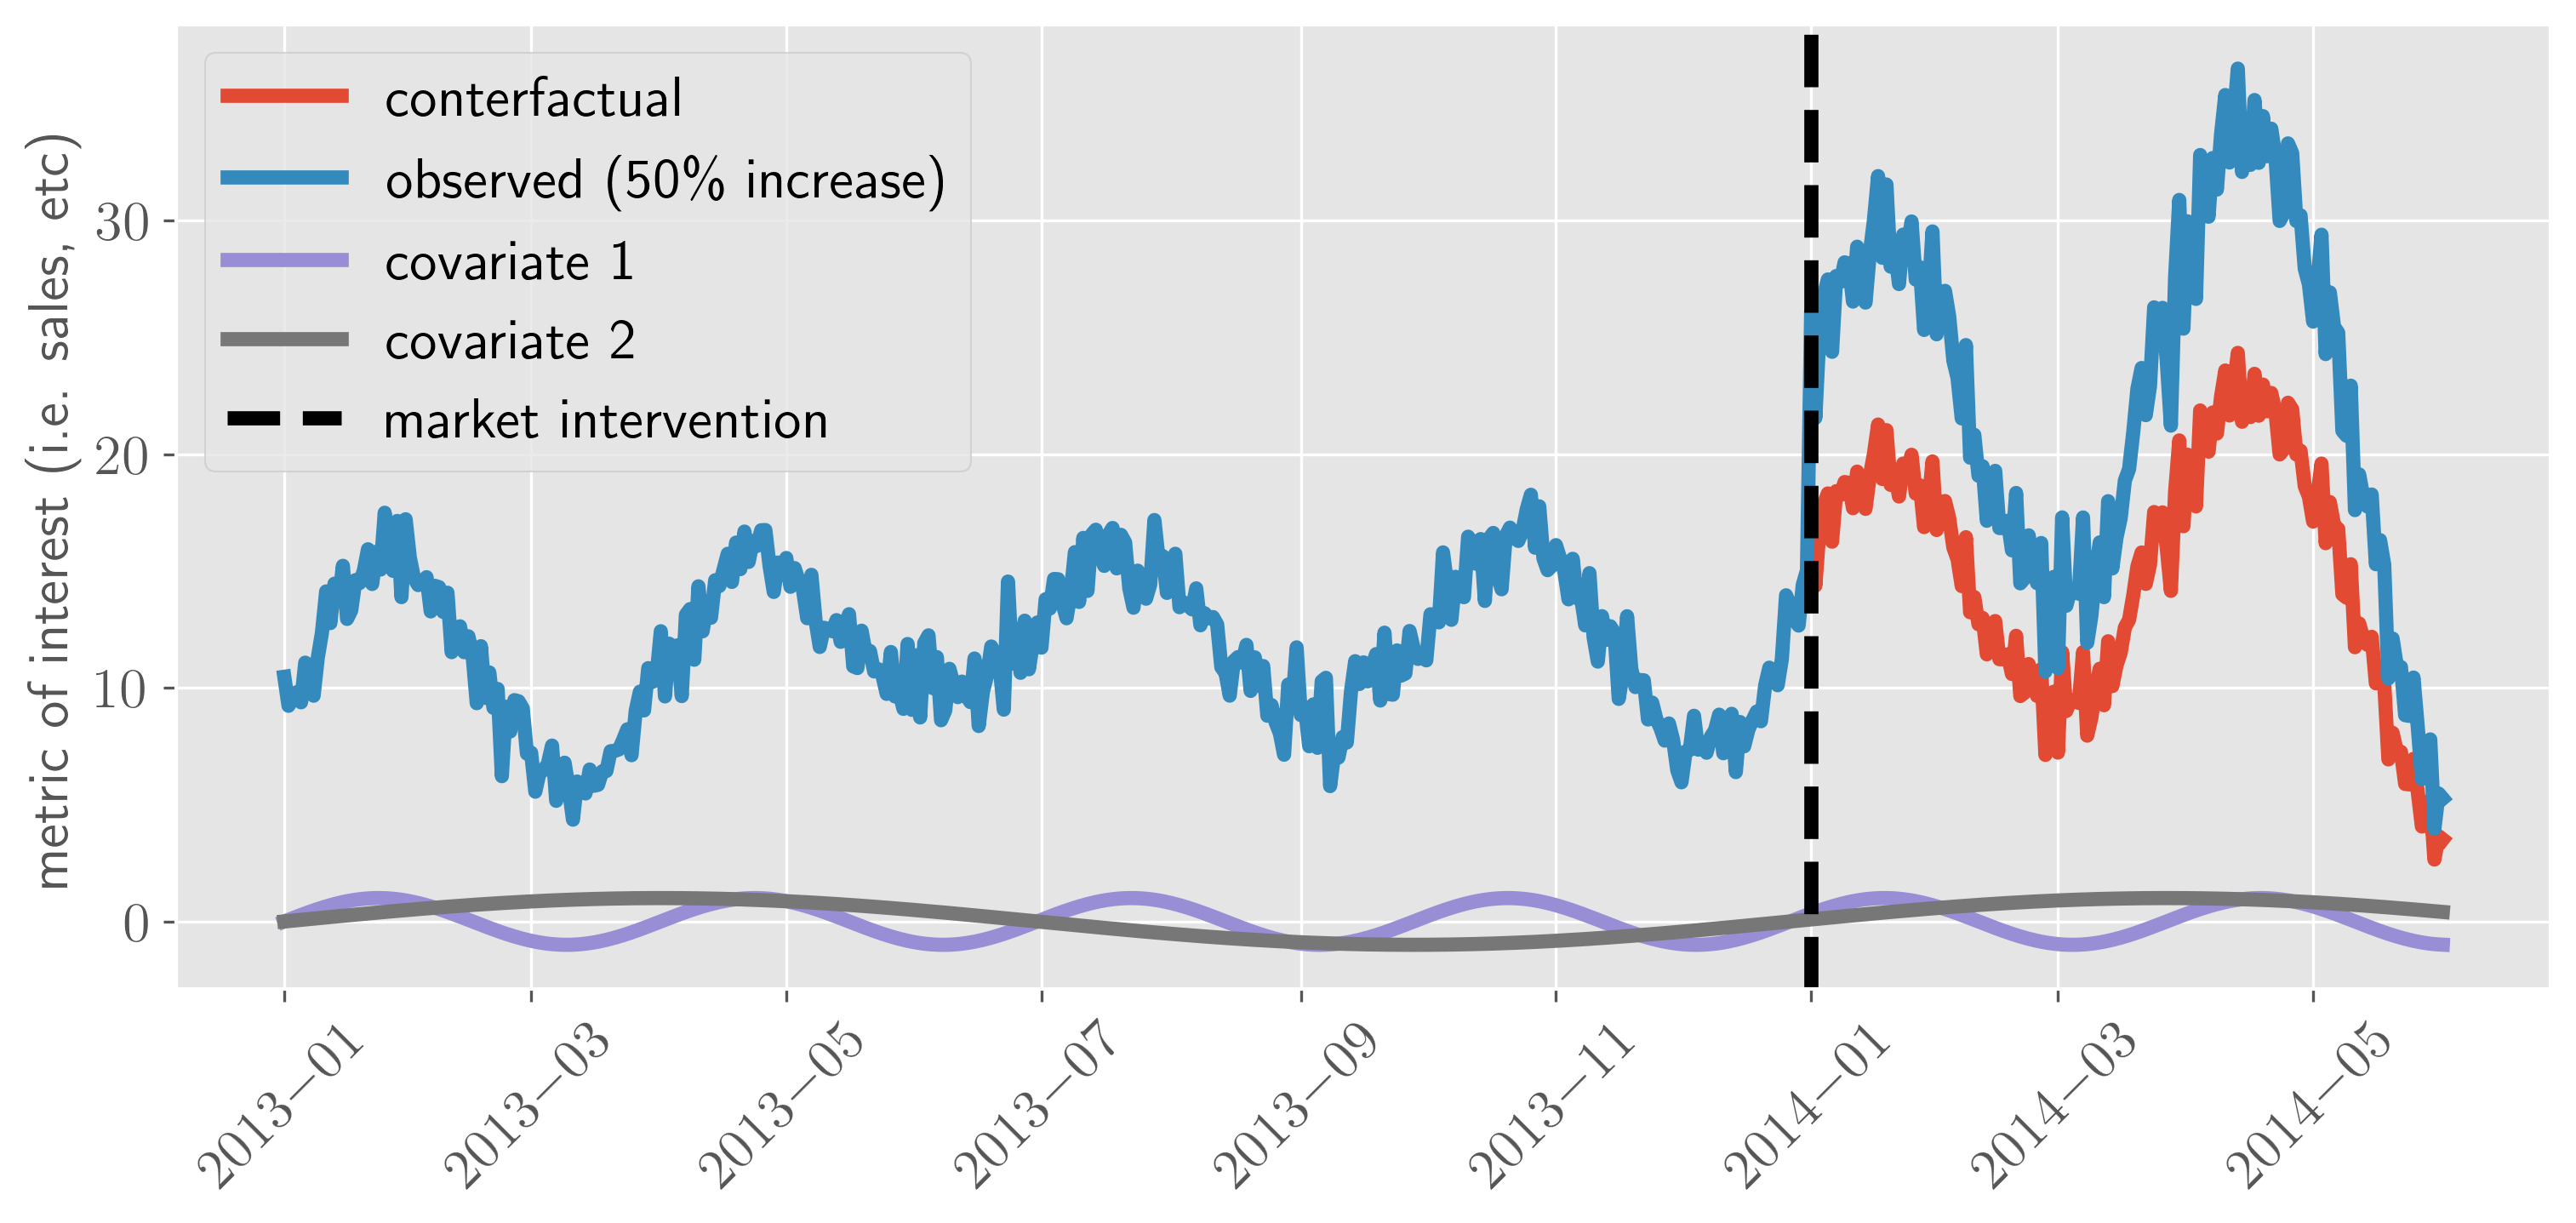
\includegraphics[scale=.6
    ]{../figures/data.png}
    \caption{Simulated data.}
    \label{data}
\end{figure}


\newpage

\subsection{Kalman Smoothing}
I used the Kalman filtering/smoothing/forecasting steps described in section \ref{kalman} to predict the counterfactual time series. Figure \ref{states} shows the states $\boldsymbol{\alpha}$ recovered by Kalman filtering alone and with Kalman smoothing.


\begin{figure}[!h]
    \centering
    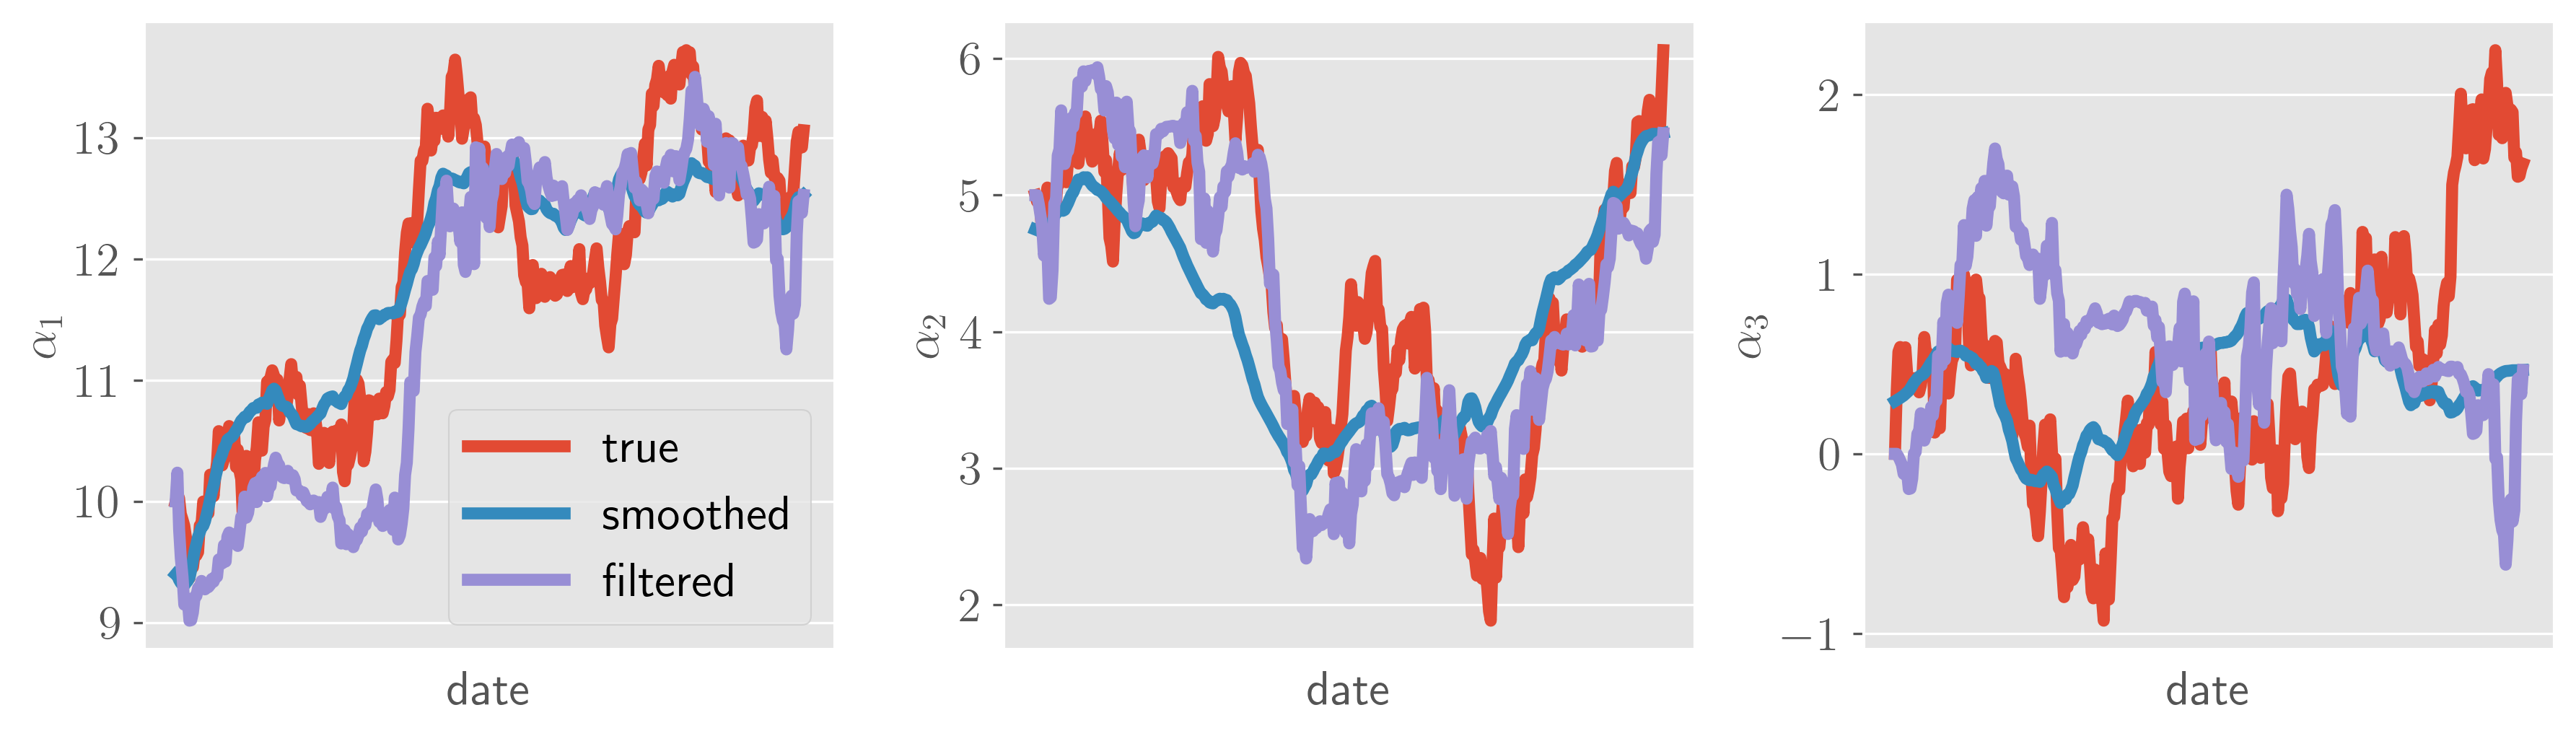
\includegraphics[scale=.5
    ]{../figures/states.png}
    \caption{States $\boldsymbol{\alpha}$ found with Kalman filtering only and Kalman smoothing. }
    \label{states}
\end{figure}

Using the results from the Kalman smoothing algorithm, the  counterfactual series was predicted as shown in Figure \ref{pred}. The absolute causal impact, defined as the difference between the observed and predicted time-series, is shown in Figure \ref{diff}.
\begin{figure}[!h]
    \centering
    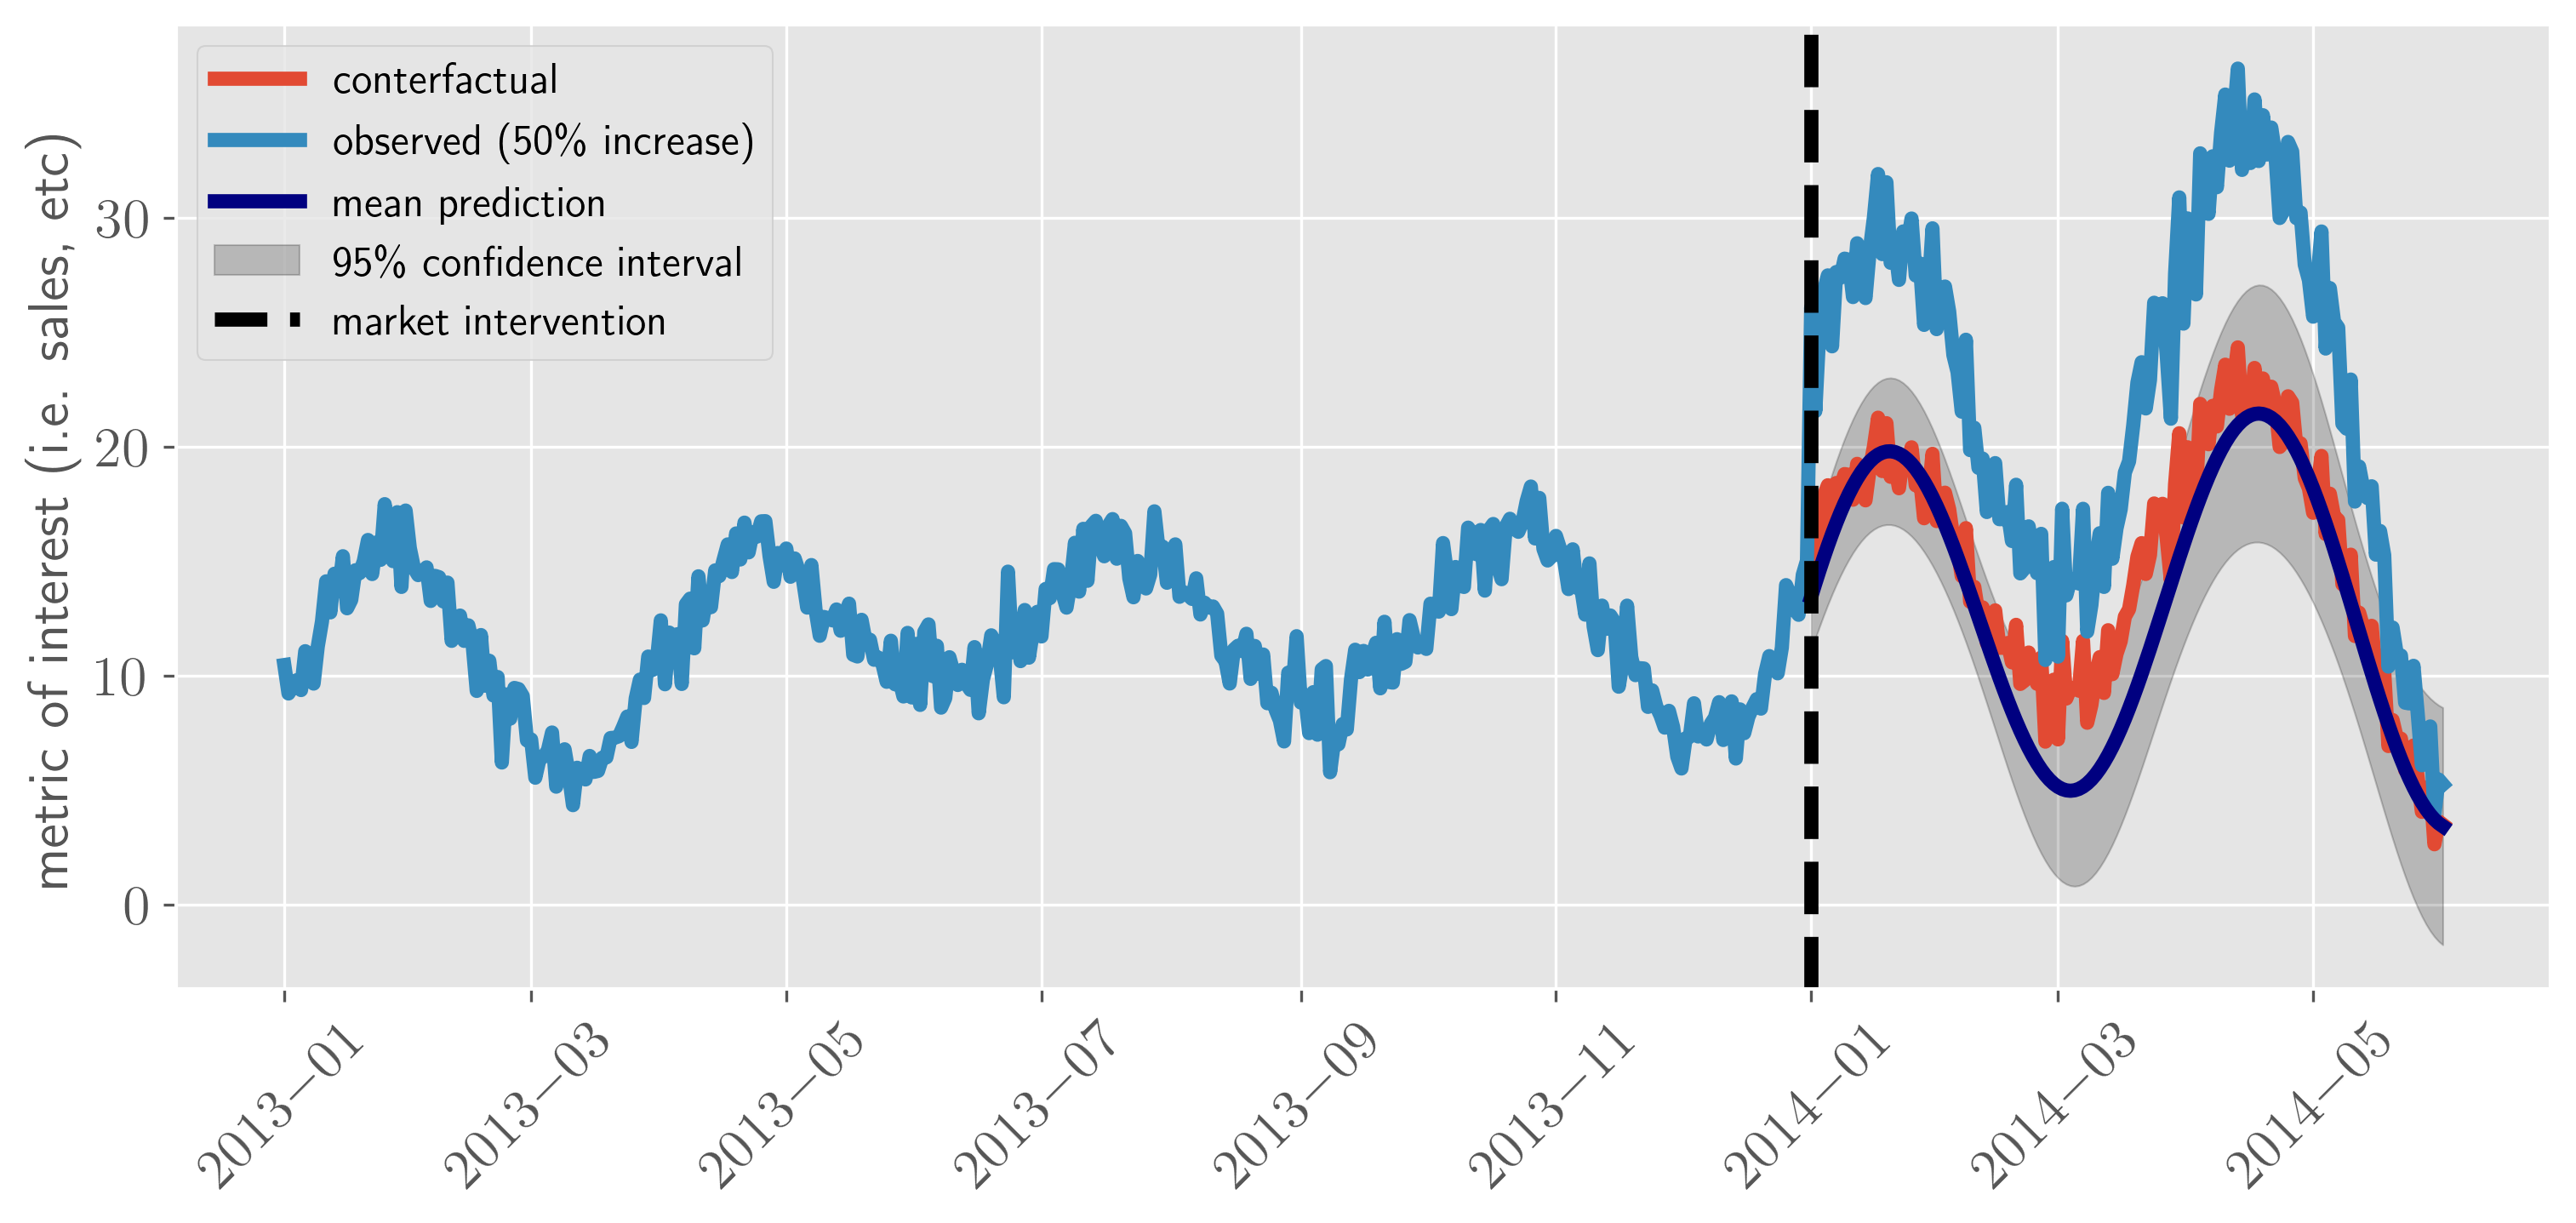
\includegraphics[scale=.5
    ]{../figures/pred.png}
    \caption{Predicted counterfactual time-series.}
    \label{pred}
\end{figure}

\begin{figure}[!h]
    \centering
    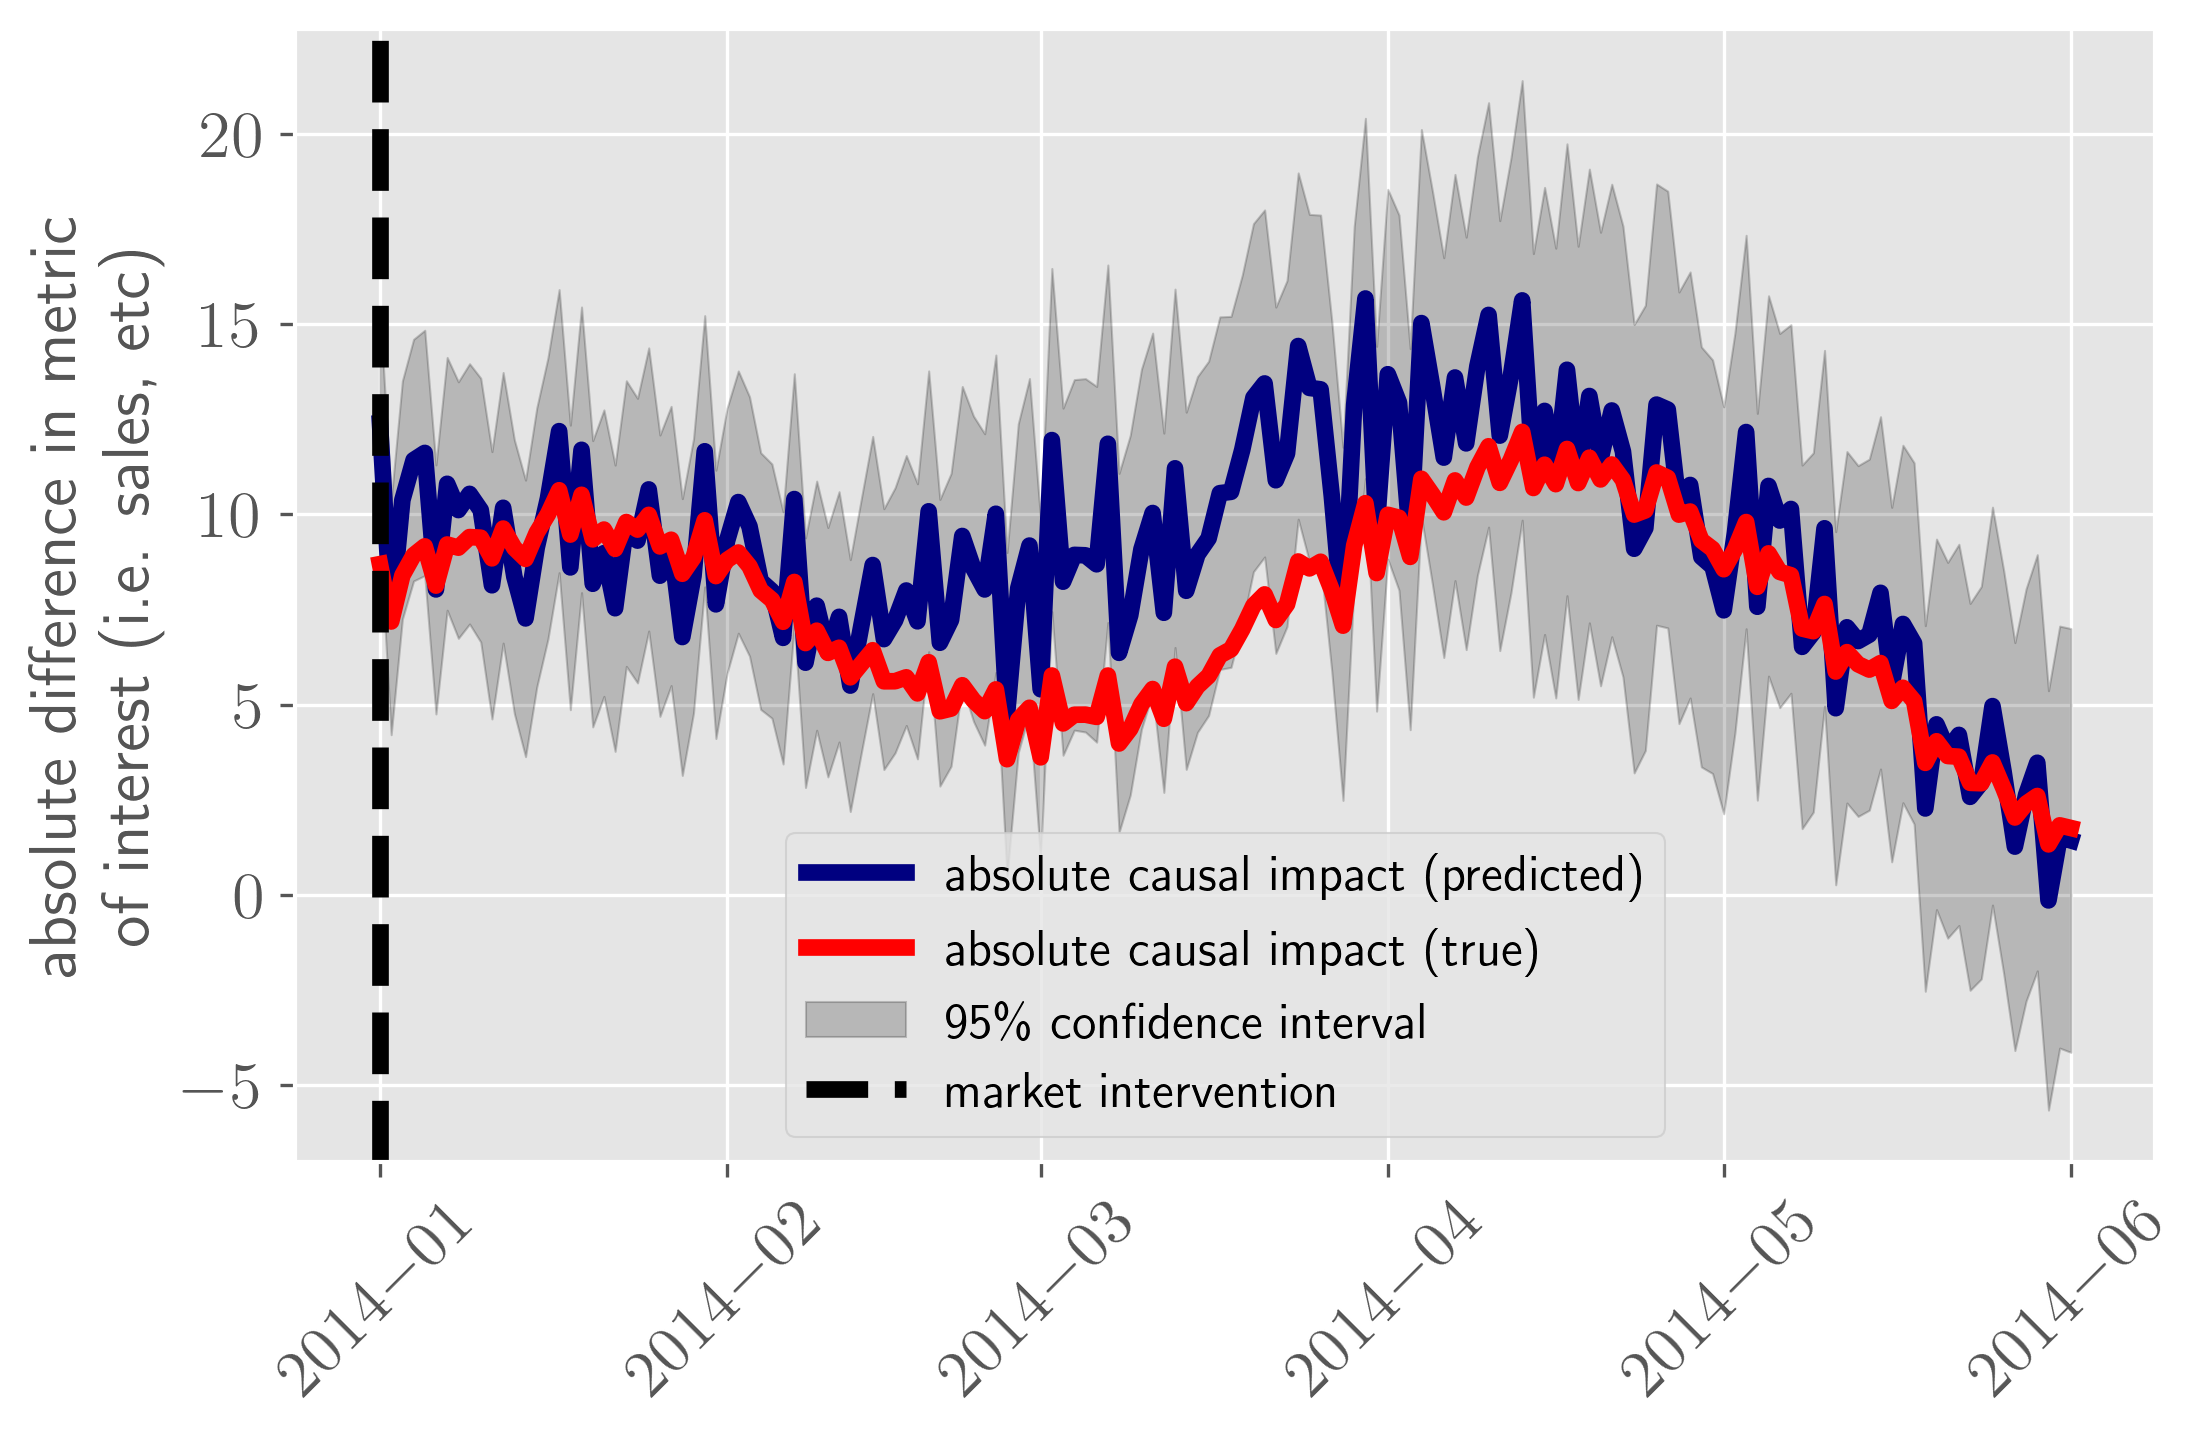
\includegraphics[scale=.5
    ]{../figures/diff.png}
    \caption{Predicted vs.\ actual absolute causal impact.}
    \label{diff}
\end{figure}
\newpage
As mentioned, I assumed that all the parameters were known in the Kalman smoother. I did attempt to infer $\sigma^2$ (which was set equal to 1) with a Gibbs sampler, which resulted in Figure \ref{sig}. I could not get the full Gibbs sampler (with all unknown parameters) to work, however.

\begin{figure}[!h]
    \centering
    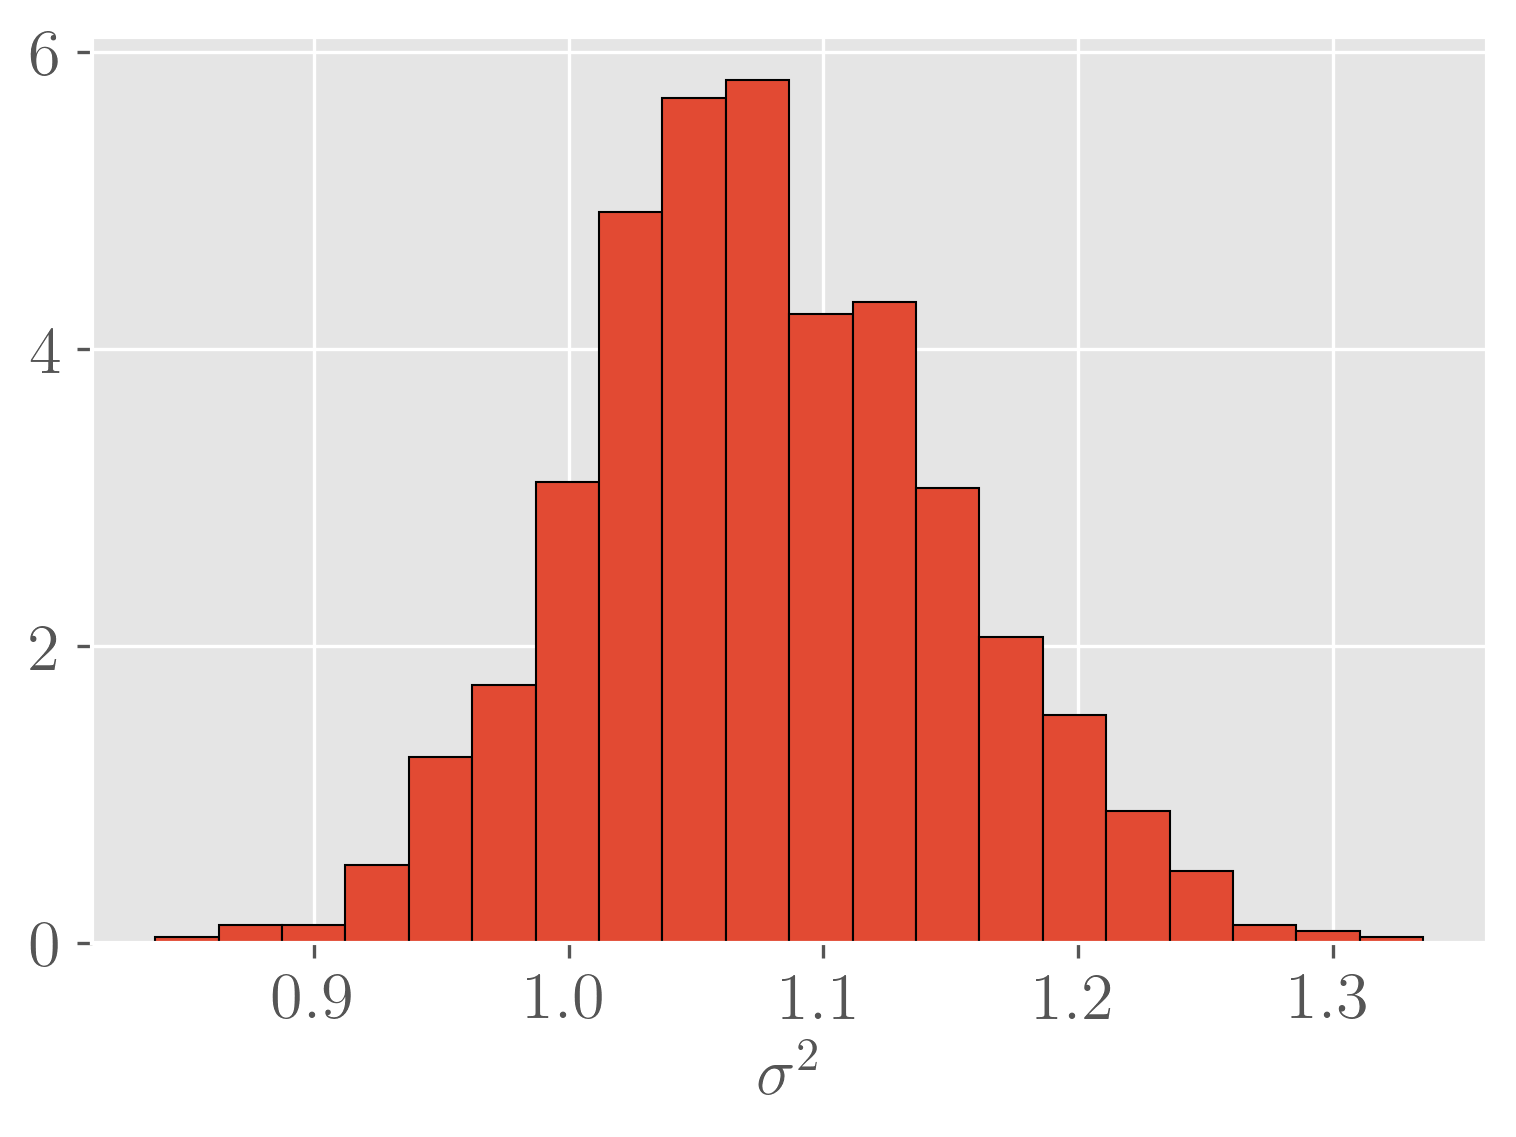
\includegraphics[scale=.6
    ]{../figures/sigma.png}
    \caption{Histogram of traces for $\sigma^2$.}
    \label{sig}
\end{figure}
\newpage

\subsection{Results}
For the rest of this section, I used the BSTS package that the authors wrote in R. In their results section for the simulated data, the authors were primarily concerned with 1) showing the relationship between effect size and the probability that the model will detect an effect and 2) showing that the proportion of simulations that predict an effect size interval containing the true effect size does not vary with campaign duration (i.e. the length of the market intervention). The sections below show how I proceeded to replicate those results.

\subsubsection{Relationship Between Effect Size and Probability of Detection}
For this section, the steps involved were:
\begin{itemize}
    \item Create datasets for various effect sizes: 0, 0.1\%, 1\%, 10\%, 25\%, 50\%, 100\%. For each effect size, $2^8$ time-series were created, using the same process as in \ref{dataset}.
    \item For each time-series, the BSTS package (configured with a local level and two dynamic regressions) was used to predict the counterfactual time-series.
    \item For each simulation, if the 95\% confidence interval for mean absolute causal impact did not contain 0, the model was deemed to have detected an effect.
    \item The last step was to plot the percentage of simulations where an effect was detected as a function of effect size.
\end{itemize}



Figure \ref{result} shows the percentage of simulations where an effect was detected as a function of effect size. The plot is very similar as the one obtained by the authors. As expected, the model is rarely able to detect an effect when the effect size is very small. As it increase, the model is almost always able to detect the effect. 
\subsubsection{Coverage Properties of the Posterior Probability Intervals as a Function of Campaign Length}
The aim of the second analysis was to show that the percentage of simulations that contained the true effect size for a given effect size did not vary as a function of campaign length. To accomplish this, the steps were:
\begin{itemize}
    \item Create datasets with varying campaign lengths. I created $2^8$ datasets for each campaign length, for campaign lengths varying from 25 to 150 days.
    \item For each dataset, I fit a BSTS model using the package
    \item For each simulation, I determined whether the true relative effect size fell into the $95\%$ CI for the predicted (average) relative effect size
    \item I plotted the percentage of intervals that contained the true effect size as a function of campaign length
\end{itemize}
The resulting plot is shown in Figure \ref{int}. Again, the plot is very similar to the plot in the paper. 

\section{Example with Real Data }
Unfortunately, the data in this section was not publicly available. The dataset that the authors used consisted of treatment and control time-series for ``number of clicks''. The treatment received was an advertising campaign. One of the main takeaways from this section was that in the absence of control time-series (i.e. data from control groups such as data from other countries/regions without market intervention), other types of time-series can be used. In the example, the authors used keyword searches from the advertiser's industry as covariates. This analysis almost perfectly replicated the analysis where the used control groups as covariates.


\clearpage
\bibliographystyle{ieeetr} 
\bibliography{ref}
\end{document}
